\subsubsection{Sid Meier's Civilization}
Das 1991 erschienene Spiel \textit{Sid Meier's Civilization} ist ein von \textit{MicroPose} entwickeltes und publiziertes, rundenbasiertes Strategiespiel \cite*[]{civigdb}. \textit{MicroPose} ist ein 1982 von Bill Stealey und Sid Meier gegründetes Softwareunternehmen, wovon von letzterem auch der Name abgeleitet wird \cite*[]{civhistory}. Man startet im Jahr 4000 B.C. und bewegt sich zeitlich bis ins Informationszeitalter, während man neue Städte gründet, Technologien erforscht und anderen Gegenspielern beziehungsweise Reichen und deren Herrschern begegnet, Diplomatie führt und gegebenenfalls auch Kriege. Unter den spielbaren Herrschern sind unter anderem \textit{Alexander der Große, Napoleon} und \textit{Julius Cäsar}. Das Spiel besitzt einen nicht-linearen Technologiebaum mit den wichtigsten Errungenschaften der Menschheit, darunter das Rad oder Navigation, verschiedene baubare Wunder, zum Beispiel die Pyramiden oder die Große Mauer und besitzt fünf verschiedene Schwierigkeitsgrade, mit denen der Spieler die Herausforderung selber setzen \cite*[]{civ}. Je nach Fokus des Spielers ist also jedes Match ein neues, und es gibt durch verschiedene Ressourcen und Entscheidungsmöglichkeiten einige Strategien denen sich der Spieler bedienen kann. \\
Das Spiel erhielt fünf weitere Nachfolger \textit{Civilization II, Civilization III, Civilization IV, Civilization V} und \textit{Civilization VI} \cite*[]{civall}, wobei sich manche Teile stark von anderen Unterscheiden, etwa in der Perspektive oder der Geometrie des Spielfeldes. So wurde von \textit{Civilization IV} auf \textit{Civilization V} das Spielfeld von einem \textit{Square Grid} auf ein \textit{Hex Grid} umgestellt \cite*[]{civallcompare}. Neben den Nachfolgern gab es einige Ableger, darunter \textit{Sid Meier's Civilization: Beyond Earth}, welches 2014 erschien und zwei Erweiterungen erhielt. Dieser Teil spielt, anders als alle anderen, auf einem fremden Planeten und hat eine Sci-Fi Thematik, statt wie üblich, eine historische \cite*[]{civbe}. Das Spiel besitzt, im Gegensatz zu allen anderen Nachfolgern, noch eine Vogelperspektive, statt wie später, eine isometrische (vgl. \autoref{image:civ}). Außerdem sind auch politische Auswahlmöglichkeiten wie Regierungen, oder religiöse Auswahlmöglichkeiten vorhanden. Die wichtigsten Eigenschaften sind in \autoref{table:civ} zusammengefasst.



\paragraph*{Siegbedingungen}
\begin{itemize}
    \item Alle Gegenspieler eliminieren mittels Militär
    \item Ein Raumschiff bauen und Alpha Centauri als erster erreichen
    \item Überleben bis die Zeit ausgelaufen ist \cite*[]{civwin}
\end{itemize}

\paragraph*{Ressourcen}
\begin{itemize}
    \item Kohle
    \item Fisch
    \item Wild
    \item Wild (Tundra)
    \item Edelsteine
    \item Gold
    \item Pferde
    \item Oasen
    \item Öl
    \item Robben
\end{itemize}\cite*[]{civ:ressources}
\newparagraph{Rezensionen}
\begin{tabularx}{0.8\textwidth} { 
    | >{\raggedright\arraybackslash}X 
    | >{\centering\arraybackslash}X 
    | >{\raggedleft\arraybackslash}X | }
    \hline
    IGDB & 93\% \cite*[]{civigdb}\\
    \hline
    AllGame & 5/5 \cite*[]{civ:review:allgame}\\
    \hline
    Game Informer & 8.5/10 \cite*[]{civ:review:gameinformer}\\
    \hline
    Next Generation & 4/5 \cite*[]{civ:review:nextgeneration}\\
    \hline
\end{tabularx}

\begin{table}[]
    \centering
    \caption{Civilization Eigenschaften (\cite*[]{civallcompare,civigdb,civwin, civ:ressources})}
    \label{table:civ}
    \begin{tabular}{|l|l|}
    \hline
    Erscheinungsjahr & 1991                                                                           \\ \hline
    Entwickler       & MicroPose                                                                      \\ \hline
    Publisher        & MicroPose                                                                      \\ \hline
    Multiplayer      & Nein                                                                      \\ \hline
    Ressourcen       & Kohle, Fisch, Wild, Wild (Tundra), Edelsteine, Gold, Pferde, Oasen, Öl, Robben \\ \hline
    Siegbedingungen  & Domination, Space Race, Time                                                   \\ \hline
    Spielbare Völker & 14                                                                             \\ \hline
    Perspektive      & Vogel                                                                          \\ \hline
    Technologien     & 67                                                                             \\ \hline
    \end{tabular}
\end{table}

\begin{figure}
    \begin{center}
        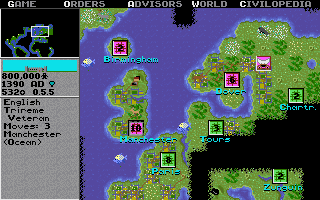
\includegraphics[width=300px]{0.bilder/civ.png}
    \end{center}
    \caption{Screenshot aus Civilization (\cite{civigdb})} \label{image:civ}
\end{figure}